The overall structure of the software system contains three layers: Camera System, Processing System, and Virtual Reality System. The Camera System is the physical hardware to get the raw video stream to transfer in the system. Also, the Camera System contains a gimbal subsystem to allow it to record video in a way that simulates the motion of a head. To make it possible to transfer the video feed across the system, the Processing System performs the necessary tasks to transfer it to the Virtual Reality System. The Virtual Reality System and the Processing System also communicate with each other in order to get the necessary head tracking angles to send to the Camera System for the gimbal subsystem.

\begin{figure}[h!]
	\centering
 	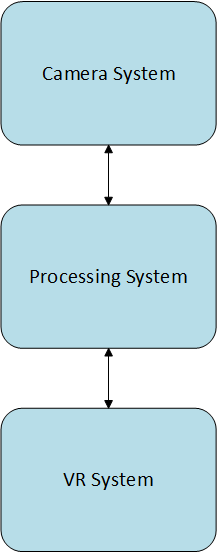
\includegraphics[width=0.2\textwidth]{images/systemoverview}
	\caption{Overall structure of system}
\end{figure}

\subsection{Camera System Layer Description}
The Camera System contains a camera subsystem, a gimbal subsystem, and a gimbal controller subsystem. The raw video stream taken from this system will be sent to the Processing System to be processed. To get the expected results from this system, the head tracking angles sent from the Processing System will be processed for this system's gimbal to read and perform accordingly.

\subsection{Processing System Layer Description}
This system contains the video input subsystem, the video output subsystem, and the gimbal controller subsystem. Raw video data will be received from the Camera System, processed, and transferred to the Virtual Reality System. In return, this system will take head tracking angles from the Virtual Reality System and send it to the Camera System through serial communication.

\subsection{Virtual Reality System Layer Description}
The Virtual Reality System is focused on delivering real-time video and tracking of the head movement on the virtual reality headset. This system contains the stereo display subsystem and the head tracking subsystem. The processed video data sent from the Processing System will be displayed in this system. At the same time, raw head tracking angles are taken from this system's headset and sent to the Processing System.